\documentclass[12pt]{article}


\usepackage{amsmath,amssymb,amsthm,enumerate,graphicx}
\usepackage{ifthen,latexsym,syntonly}
\usepackage{setspace}
\usepackage[showrefs]{refcheck}  %use this to show equation and section labels
\usepackage[round,comma,authoryear]{natbib}   % for natbib
\usepackage{subfigure}
\usepackage{float}
\usepackage{epstopdf}
\usepackage{bm}
\usepackage{soul}

%commands to allow for easy editing
\usepackage[usenames,dvipsnames]{color}

%command to insert editing comments or track changes
\newcommand{\dge}[1]{\textcolor{blue}{$^{\textrm{dge}}${#1}}}
\newcommand{\apb}[1]{\textcolor{magenta}{$^{\textrm{apb}}${#1}}}
\newcommand{\tjs}[1]{\textcolor{red}{$^{\textrm{tjs}}${#1}}}

\bibliographystyle{mynat}


\onehalfspacing


   % for natbib
%\bibpunct{(}{)}{,}{a}{}{,}  % for natbib
%                            % need to have mynat.bst in an accesssible directory


\bibpunct{(}{)}{,}{a}{}{,}  % for natbib
                            % need to have mynat.bst in an accesssible directory

\newcommand{\EE}{\mathbb E}
\newtheorem{theorem}{Theorem}[section]
\newtheorem{remark}[theorem]{Remark}
\newtheorem{assumption}[theorem]{Assumption}
%\newtheorem{case}[theorem]{Case}
\newtheorem{claim}[theorem]{Claim}
%\newtheorem{conclusion}[theorem]{Conclusion}
\newtheorem{corollary}[theorem]{Corollary}
\newtheorem{condition}[theorem]{Condition}
\newtheorem{criterion}[theorem]{Criterion}
\newtheorem{definition}[theorem]{Definition}
\newtheorem{example}[theorem]{Example}
\newtheorem{lemma}[theorem]{Lemma}
\newtheorem{problem}[theorem]{Problem}
\newtheorem{proposition}[theorem]{Proposition}
%\newtheorem{solution}[theorem]{Solution}
%\newtheorem{summary}[theorem]{Summary}
\newtheorem{thm}[theorem]{Theorem}



\setlength{\oddsidemargin}{.05in} \setlength{\topmargin}{-.45in}
\setlength{\textwidth}{6.4in} \setlength{\textheight}{8.5in}


%\pagestyle{empty}

\title {Optimal Taxation with Incomplete Markets}
%\author{Anmol Bhandari, David Evans, Mikhail Golosov, Thomas J. Sargent}
\author{\textbf{Anmol Bhandari}\\apb296@nyu.edu \and \textbf{David Evans} \\ \texttt{dgevans@nyu.edu} \and \textbf{Mikhail Golosov}\\\texttt{golosov@princeton.edu} \and \textbf{Thomas J. Sargent} \\ \texttt{thomas.sargent@nyu.edu}
}

\begin{document}

\maketitle



\begin{abstract}

\end{abstract}


\noindent\textsc{Keywords:}
\begin{quote}
``$\ldots$ the option to issue state-contingent debt is important: tax policies that
are optimal under uncertainty have an essential `insurance' aspect to them.'' \quad \citet[p.~XXXX]{LucasJr.1983}
\end{quote}
\section{Introduction}


 


Recent controversies surrounding \citet{Reinhart2010} motivated us to reconsider what we know and don't know about two elementary questions.
What is an optimal  government debt? And  is government debt  an independent state variable in a recursive formulation of a Ramsey problem?  


\citet{LucasJr.1983} and \citet{Aiyagari2002} offer  different answers to these
questions in the context of  economic environments that are identical in all respects but one: \citet{LucasJr.1983} allow the government to issue
a complete set of Arrow securities, while   \citet{Aiyagari2002} allow it to issue only a one-period risk-free government bond.  For 
\citeauthor{LucasJr.1983}, under an optimal policy  government debt is not an independent state variable but an exact function of 
 a Markov state variable that  drives government expenditures.  The optimal state-by-state levels of government debt  depend on the initial
 government debt.  By way of contrast, for \citet{Aiyagari2002} government debt is an independent state variable with a limiting value or distribution
 of values that does not depend on the initial government debt.  The quote by \citeauthor{LucasJr.1983} pinpoints the source of these differences:
 the government's purchase of {\em insurance} from the private sector  through explicit state-contingent securities underlies \citeauthor{LucasJr.1983}'s
 answers to our two questions; while a government's {\em self-insurance} by holding a risk-free asset underlies \citeauthor{Aiyagari2002}'s answers.
  
This paper revisits  our two questions in the context of a generalization of the \citet{Aiyagari2002} environment that continues to restrict
the government to issue only a single security, but sometimes makes the exogenous payoff on that security risky.  The  government
must cope as best it can with the security it is allowed to issue.  We study the implications of alternative exogenous securities for government debt dynamics.  We use this generalization of \citeauthor{Aiyagari2002}'s setup to attack questions left unresolved by \citeauthor{Aiyagari2002}
and in addition to say more things about how the government achieves  the insurance in an equilibrium in the original    \citet{LucasJr.1983}
model. Our analysis exploits  new or at least previously unstated connections between the \citeauthor{LucasJr.1983} and \citeauthor{Aiyagari2002} economies.

\citeauthor{Aiyagari2002} obtained their sharpest results for an economy with a quasi-linear household one-period utility function.
 That linearity of utility in consumption tied down the risk-free one-period interest rate enabled them to attain their result that in the long run the government accumulates a big enough stock of the risk-free asset entirely to finance its expenditures from interest earned from its claims
 on the private sector, so the tail of the Ramsey plan exhibits a zero distorting tax on labor and a first-best allocation.  
\citeauthor{Aiyagari2002} were able to say much less for preferences that exhibit risk-aversion in consumption because then the Lagrange multiplier
on the key incomplete markets implementability constraint becomes a risk-adjusted martingale rather than the martingale that it is under quasi-linearity.  Here we are able to say much more  than \citeauthor{Aiyagari2002}. We accomplish this by recognizing connections to limits of (our generalization of)
their economy and the allocation associated with a \citeauthor{LucasJr.1983} economy for a particular initial level of government debt.  
With preferences that exhibit risk aversion in consumption, an attractor for the limiting debt dynamics of our economy is not associated with  the first-best
allocation  active for the quasi-linear economy of \citeauthor{Aiyagari2002} but rather an allocation associated with a Lucas-Stokey economy or one close to it.

Our analysis sheds light on the risk-sharing theme in the quotation with which we begin this paper. We  exploit insights about exactly {\em how} the Ramsey planner
in a Lucas-Stokey economy delivers the insurance through state-contingent debt that Lucas and Stokey stress is part and parcel of an optimal tax plan:  fluctuations in
 equilibrium interest rates do part of the job.  We can construct examples in which the Lucas-Stokey Ramsey planner chooses to issue risk-free debt and to
 achieve the required state-contingencies entirely through equilibrium fluctuations in the risk-free rate of interest rate.
 
The heart of our analysis is first to find the tail of an   incomplete markets Ramsey allocation, then to ask whether that long-run allocation coincides with a Lucas-Stokey complete markets Ramsey allocation for {\em some} initial government debt.  We describe conditions in which the
answer is `yes' or `almost'.  

The structure of our analysis is related to but differs from   inquiries of \citet{Angeletos}, \citet{Buera_Nicolini}, and \citet{Shin2007}. Like us, they  want understand the link between state-contingent government  debt and an optimal tax plan. They  begin with a Lucas-Stokey complete market  Ramsey allocation
and study how it  can be supported by  a limited  collection of non-contingent debts of different maturities. Equilibrium interest rate fluctuations
let state-contingent returns help. 

In addition to the intrinsic interest that we attach to the two questions with which we began, this paper can be viewed as
a prolegomenon to an an analysis of debt dynamics in a more complicated   economic environment featured in \citet{BEGS1}.  There
a Ramsey planner levies a distorting tax on labor partly to finance exogenous government  and partly to redistribute among heterogeneously skilled households.
Debt dynamics are driven by some forces similar to those present in the simpler environment of this paper, but they are obscured by 
additional features.  We find it enlightening to study the underlying forces in a simpler setting.

\section{Environment}



We analyze economies that share the following features.
Government expenditures at time $t$, $g_t=g(s_t)$, and a productivity shock $\theta_t=\theta(s_t)$ are both functions of
  a Markov  shock $s_t\in \mathcal{S}$ having  $S \times S$ transition matrix $\Pi$ and initial condition $s_{-1}$. We will denote time $t$ histories with $s^t$ and $z_t$ will refer to a generic random variable measurable with respect to $s^t$. Sometimes we will denote $z_t(s^t)$ indicate a particular realization of $z_t$.
   %; $g_t=g(s_t);\theta_t=\theta(s_t)$
 An infinitely lived representative consumer has preferences over allocations  $\{c_t, l_t\}_{t=0}^\infty$ of consumption and labor supply that are ordered
by
   \begin{equation}
   \label{eqn:obj}
\mathbb{E}_{-1}\sum_{t=0}^{\infty } \beta^t  U\left(
c_t,l_t\right)
\end{equation}%
\dge{Where $U$ is the period utility function for consumption and labor.  For most of the paper we will assume $U$ separable in consumption and labor.  Additional assumptions will be made as needed.}  Labor produces output via the linear technology
  \begin{equation*}
  y_t=\theta_{t} l_{t} \end{equation*}
The representative consumer's tax bill
 at time $t \geq 0$ is
 \[- T_t + \tau_t \theta_{t}l_{t},  \ T_t \geq 0, \]
 where $\tau_t(s^t,)$ is a flat rate tax on labor income and $T_t$ is a nonnegative transfer.
 Often, we'll set $T_t =0$.
The government and consumer trade a single  possibly risky  asset whose  time $t$ payoff $p_t$ is described by an $S \times S$ matrix $\mathbb{P}$:
%\[p_t=\st{\mathbb{P}(s_{t}|s_{t-1})} \]
\[p_t=\mathbb{P}(s_{t},s_{t-1}) \]

Let $B_t$ denote the government's holdings of the asset and $b_t$ be the consumer's holdings.
Let $q_t= q_t(s^t)$ be the price of the single  asset at time $t$.
 At $t \geq 0$, the household's time budget constraint is
 \begin{equation}
 \label{eqn:HHbudget}
 c_{t}+b_{t}=\left( 1-\tau _{t}\right) \theta _{t}l_{t}+\frac{p_{t}}{q_{t-1}}b_{t-1}+T_{t}
 \end{equation}

 and the government's is
 \begin{equation}
 \label{eqn:Govbudget}
g_{t}+B_{t}+T_t=\tau _{t}\theta_{t}l_{t}+\frac{p_{t}}{q_{t-1}}B_{t-1}.
 \end{equation}


Feasible allocations satisfy

\begin{equation}
 \label{eqn:ResFeas}
 c_{t}+g_t = \theta _{t} l_{t}, \ \forall t \geq 0
 \end{equation}

 Clearing in the time $t \geq 0$ market for the single asset requires

 
\begin{equation}
 \label{eqn:bondmarket}
 b_{t}+B_{t}=0.
 \end{equation}

 Initial assets satisfy $b_{-1}=-B_{-1}$\footnote{\apb{We assume that $b_{-1}$ are obligations with acrrued interest. This is equivalent to setting $q_{-1}=1$}} An initial value of the exogenous state  $s_{-1}$ is given.
Equibrium objects including $\{c_t, l_t, \tau_t\}_{t=0}^\infty$ will come in the form of sequences of functions of  initial government debt  $b_{-1}$ and  $s^t = [s_t, s_{t-1}, \ldots, s_0, s_{-1}]$.


Borrowing from a standard boilerplate, we use the following:

\begin{definition}
An \textbf{allocation} is a sequence $\{c_t,l_t\}_{t=0}^\infty$ for consumption and labor. \dge{An \textbf{asset profile}  is a sequence $\{b_t,B_t\}_{t=0}^\infty$}. A \textbf{price system} is a sequence of asset prices $\{q_t\}_{t=0}^\infty$.  A \textbf{budget-feasible government policy} is a sequence of taxes and transfers $\left\{ \tau _{t},T_{t}\right\} _{t=0}^{\infty }$
\end{definition}

\begin{definition}
Given  $\left(b_{-1}=-B_{-1},s_{-1}\right) $ and a government policy,  a \textbf{competitive equilibrium
with distorting taxes} is a price system, \dge{an asset profile}, a \st{budget-feasible} government policy, and an allocation such that
the allocation maximizes \eqref{eqn:obj} subject to \eqref{eqn:HHbudget} \dge{and $\{b_{t}\}_{t=0}^\infty$ bounded}  given prices; and \st{the bond  market clears} \dge{equations \eqref{eqn:Govbudget}, \eqref{eqn:ResFeas} and \eqref{eqn:bondmarket} are satisfied}.
\end{definition}

\begin{definition}
Given $\left( b_{-1},B_{-1},s_{-1}\right) $, a \textbf{Ramsey plan} is a welfare-maximizing competitive
equilibrium with distorting taxes.
\end{definition}


\section{Two Ramsey problems}

Following \citet{LucasJr.1983}
and
\citet{Aiyagari2002}, we use a
``primal approach.''   To encode a  government policy and price system as a restriction on an allocation,
we  first obtain   the representative household's first order conditions\footnote{We thus focus on interior equilibria. \dge{Arguments in \cite{Magill1994} and \cite{Constantinides1996} can be used to show that any allocation $c_t$, $l_t$, $b_t$ that satisfy equations \eqref{eqn:HHbudget},\eqref{eqn:HHFOC} and bounded $\{b_t\}$ is a solution to the consumers problem.} }
\begin{subequations}\label{eqn:HHFOC}
	\begin{equation}
	\label{eqn:Euler}
		U_{c,t} q_t = \beta \EE_t p_{t+1}U_{c,t+1} 
	\end{equation}
	\begin{equation}\label{eqn:lcFOC}
		(1-\tau_t)\theta_tU_{c,t} = - U_{l,t} 
	\end{equation}


\end{subequations}
We substitute these into the household's budget constraint to get a difference equation that we  solve forward   at every history for every $t \geq 0$.
That yields \textit{implementability constraints} on a Ramsey allocation that fall into two categories: (1) the time $t=0$ version is identical
with the {\em single} implementability constraint imposed by \citet{LucasJr.1983}; (2) the time $t \geq 1$ implementability constraints
are counterparts  of the additional
 \emph{measurability restrictions} that \citet{Aiyagari2002} impose on  a Ramsey allocation.
%
%\item[4.]  \textbf{Transfers: } We temporarily restrict transfers $T_t = 0$  $\forall t$. This is convenient for our analytical results.  We eventually show  that this assumption is not restrictive.
% \end{enumerate}





%
%The primal approach version of
%\begin{equation*}
%\max_{\{c_t,l_t\}} \EE_0\sum_{t=0}^\infty \beta^t U(c_t,l_t)
% \end{equation*}
% subject to
%
% \vspace{3mm}
%
% (a) \textbf{Feasibility}
%\begin{subequations}
%\begin{equation*}
%c_t + g_t = \theta_t l_t
% \end{equation*}
%
%(b) \textbf{Implementability constraint}
%
%% \begin{equation*}
%% \frac{b_{t-1}U_{c,t-1}}{\beta} = \frac{\EE_{t-1} p_t U_{c,t}}{p_t U_{c,t}}\EE_t\sum_{j=0}^\infty\beta^j\left( U_{c,t+j}c_{t+j}+U_{l,t+j}l_{t+j}\right)\text{  for $t\geq 1$ }
%% \end{equation*}
%\begin{equation*}
%b_{-1} = \frac1{U_{c,0}}\EE_0\sum_{t=0}^\infty \beta^t\left(U_{c,t}c_t+U_{l,t}l_t\right)
% \end{equation*}
%\end{subequations}
We first state our Ramsey problem, then Lucas and Stokey's.




\begin{problem}\label{prob:RamseyBEGS}
The  Ramsey problem is to choose an allocation and an \st{appropriately measurable}\dge{bounded} government debt sequence $\{b_t\}_{t=0}^\infty$ %sequences  functions
%$\{c_t(s^t),l_t(s^t), b_t(s^t)\}_{t=0}^\infty$
that attain:
\begin{equation}\label{eqn:Ramseyobj}
\max_{\{c_t,l_t,b_t\}} \EE_0\sum_{t=0}^\infty \beta^t U(c_t,l_t)
 \end{equation}
subject to
% \vspace{3mm}
%
% (a) \textbf{Feasibility}
\begin{subequations}
\begin{equation}\label{eqn:feas}
c_t + g_t = \theta_t l_t, \ t \geq 0
 \end{equation}

%(b) \textbf{Lucas-Stokey implementability constraint}
\begin{equation}\label{eqn:LSimplement}
b_{-1} = \frac1{U_{c,0}}\EE_0\sum_{t=0}^\infty \beta^t\left(U_{c,t}c_t+U_{l,t}l_t\right)
 \end{equation}

 %(c) \textbf{Measurability constraints}
 \begin{equation}\label{eqn:AMSSimplement}
 \frac{b_{t-1}U_{c,t-1}}{\beta} = \frac{\EE_{t-1} p_t U_{c,t}}{p_t U_{c,t}}\EE_t\sum_{j=0}^\infty\beta^j\left( U_{c,t+j}c_{t+j}+U_{l,t+j}l_{t+j}\right)\text{  for $t\geq 1$ }
 \end{equation}
  
\end{subequations}
\end{problem}

\begin{problem}\label{prob:RamseyLS}
Lucas and Stokey's Ramsey problem is to choose an allocation %$\{c_t(s^t),l_t(s^t)\}_{t=0}^\infty$
that attains % the maximum of
\begin{equation}\label{eqn:RamseyobjLS}
\max_{\{c_t,l_t\}} \EE_0\sum_{t=0}^\infty \beta^t U(c_t,l_t)
 \end{equation}
 subject to the single implementability constraint \eqref{eqn:LSimplement} and feasibility \eqref{eqn:feas} for all $t, s^t$.
\end{problem}

\begin{remark} Equation \eqref{eqn:feas} imposes feasibility, while equation  \eqref{eqn:LSimplement} is the single implementability constraint
present in \citet{LucasJr.1983}.  Equations \eqref{eqn:AMSSimplement} express  additional \st{implementability constraints that comprise} implementability constraints at every node from time $t \geq 1$. These generalize the \citet{Aiyagari2002} measurability constraints on a Ramsey allocation  to our more general payoff structure ${\mathbb P}$ for the
single asset. The measurability constraints \eqref{eqn:AMSSimplement}  are cast
in terms of the date, history $(t-1, s^{t-1})$ measurable state variable $b_{t-1}$ that for $t \geq 1$ is absent from Lucas and Stokey's complete markets Ramsey problem.  Evidently, Ramsey allocation for our incomplete markets economy automatically satisfies the single implementability constraint imposed by \citeauthor{LucasJr.1983}.
\end{remark}


\begin{remark}\label{rem:LSdebt}
State-contingent, but not history-dependent,  values of consumption, labor supply, and continuation government debt $\check b(s)$ solve the \citet{LucasJr.1983} Ramsey problem \ref{prob:RamseyLS}.  As intermediated by the Lagrange multiplier on the implementability constraint \eqref{eqn:LSimplement},
consumption, labor supply, and $\check b(s)$ are  functions of initial government debt $b_{-1}$ and the current state $s_t$, but not past history $s^{t-1}$.
\end{remark}

\subsection{Motivation for  quasi-linear $U$\label{sec:excusequasilinear}}
Asymptotic properties of a Ramsey plan for our incomplete markets economy vary  with asset returns $R_{t-1,t}\equiv \frac{\mathbb{P}(s_{t}|s_{t-1})}{q_{t-1}}$. We see that $\mathbb{P}$ affects these returns directly through the ex-post exogenous payoffs and indirectly through prices $q_{t-1}$. To focus exclusively on the exogenous $\mathbb{P}$ part of returns, we begin  by studying an economy with  quasi-linear  utility function:
  \begin{equation}\label{eqn:UQL}
U(c,l)=c-\frac{l^{1+\gamma}}{1+\gamma},\end{equation} which sets $U_{c,t}= 1$.  Asymptotic properties of a Ramsey plan for our incomplete markets economy vary  with   asset returns that reflect
	properties of equilibrium prices $\{q_t(s^t|B_{-1},s_{-1})\}_t$ and the exogenous asset payoff matrix $\mathbb{P}$.
At an interior solution, quasi-linear preferences and the Euler equation \eqref{eqn:Euler} pins down $q_t=\beta \mathbb{E}_t
\mathbb{P}(s_{t+1}|s_t)$.  After studying the consequences of quasi-linear utility, we shall solve for Ramsey plans for utility functions that express risk aversion with respect to consumption and so activate endogenous fluctuations in $q_t$.
	


\section{Quasi-linear preferences}

Throughout this section, we assume that $U$ is quasi-linear and use an indirect three step approach to  characterize  the asymptotic behavior of government  debt and the tax rate.



\noindent (1) \textbf{Construct  an optimal payoff matrix:}

We pose the following problem:
\begin{problem}\label{prob:PPoperator}
 Given arbitrary initial government debt $b_{-1}$, what is an optimal asset payoff matrix?
\end{problem}
\noindent  \dge{Let $\mathcal P$ be the set of all $\mathcal S\times \mathcal S$ real matrices.  Define the indirect utility function $\mathcal W(\mathbb P;b_{-1})$ as the solution to problem \ref{prob:RamseyBEGS} for $\mathbb P \in \mathcal P$ and initial debt $b_{-1}$.  This induces an operator $\mathbb P^*$ that maps initial government debt into an optimal payoff matrix \footnote{\dge{We will demonstrate existence of a maximizer.  The solution will be unique up to a constant factor along each row of the matrix.}}
\[
	\mathbb P^*(b_{-1}) \in \arg\max_{\mathbb P\in \mathcal P} W(\mathbb P; b_{-1})
\] }



\noindent (2) \textbf{Apply the inverse of the operator $\mathbb{P}^*$.}

\dge{For an arbitrary payoff matrix $\mathbb{P}$,  let
\begin{equation}\label{eqn:invPoperator}\mathbb{P}^{* -1}(\mathbb{P}) =\min_{b}\|\mathbb{P}-\mathbb{P}^*(b^*)\|,
\end{equation}where $\|\cdot\|$ is the Frobenius matrix norm.  For initial government debt $b_{-1}$ such that $\mathbb P^*(b_{-1}) = \mathbb P$ we will show that Ramsey plan for the incomplete markets economy has $b_t = b^*$ for all $t \geq 0$.}


\noindent (3) \textbf{Long run assets}

Starting from an arbitrary initial government $b_{-1}$ and an arbitrary payoff matrix $\mathbb{P}$,  establish conditions under  which $b_t \to b^*$ under a Ramsey plan.


In particular, where $S=2$ and shocks $s_t$ are IID,  we describe a large set of  $\mathbb{P}$'s for which government debt $b_t$  under a Ramsey plan converges to $b^*$.  For more general shock processes, we numerically find  an ergodic set of $b_t$'s hovering around \st{a}\dge{the} debt level $b^*$.  \dge{Steps (1), (2) and (3) are executed in sections 4.1, 4.2 and 4.3.}    
\subsection{The Optimal Payoff Matrix}\apb{The optimal payoff matrix is obtained by reverse engineering a Lucas-Stokey Ramsey allocation} for a given $b_{-1}$ by solving  problem \ref{prob:RamseyLS}.\apb{Next we find a sequence $\{p_t\}_t$ that satisfies the implementability constraints imposed in \eqref{eqn:AMSSimplement}}.  Note that these implementability constraints are invariant to scaling of $p_t$ by a constant $k_{t-1} $ that can depend on $s^{t-1}$. From this equivalence class of $\{p_t\}_t$'s we select a  $\{p_t\}_t$ that imposes the normalization  \st{$\mathbb{E}_{t-1}U_{c,t}p_t=1$}\dge{$\mathbb{E}_{t-1}p_t=1$} and satisfies
\begin{equation}\label{eqn:pdisarm} 
p_t =  \frac{\beta}{b_{t-1}}\EE_t\sum_{j=0}^\infty\beta^j\left( c_{t+j}+U_{l,t+j}l_{t+j}\right) 
\end{equation}\dge{where 
\begin{equation}\label{eqn:bt-1}
	b_{t-1} = \beta \EE_{t-1}\sum_{j=0}^\infty \beta^j(c_{t+j}+U_{l,t+j}l_{t+j})
\end{equation}  The term $c_{t+j} +U_{l,t+j}l_{t+j}=(1-\tau_{t+j})l_{t+j} - g_{t+j}$ which is the net-of-interest government surplus at time $t+j$.  Combining equations \eqref{eqn:pdisarm} and \eqref{eqn:bt-1} we note that  $\frac{1}{p_t}-1$ is then the percent innovation in present value government surplus at time $t$.} 


Note that by construction, $p_t$   disarms the time  $t\geq 1$
measurability constraints\footnote{\dge{Although quasi-linear preferences are implicitly assumed during this construction.  Equation \eqref{eqn:pdisarm} can be generalized to preferences with curvature via
\[
p_t =  \frac{\beta}{U_{c,t-1}b_{t-1}U_{c,t}}\EE_t\sum_{j=0}^\infty\beta^j\left( U_{c,t+j}c_{t+j}+U_{l,t+j}l_{t+j}\right) \]
with the normalization $\EE_{t-1}U_{c,t}p_t = 1$}}.  Using the fact noted in remark \ref{rem:LSdebt} that the Lucas-Stokey Ramsey allocation is not history-dependent,  construct the optimal payoff matrix as
\[\mathbb{P}^*(s_t,s_{t-1}|b_{-1})=p_t.\]

Thus,  given
 initial government debt $b_{-1}$,  let $\mu(b_{-1})$ be the Lagrange multiplier on the Lucas-Stokey implementability constraint \eqref{eqn:LSimplement}
 at the Lucas-Stokey Ramsey allocation.   The tax rate in the Ramsey allocation is
$
		\tau(\mu) = \frac{\gamma\mu}{(1+\gamma)\mu-1},
	$
 which implies a  net-of-interest government surplus $S(s,\tau)$ that satisfies
\[		S(s,\tau) = \theta(s)^\frac\gamma{1+\gamma}(1-\tau)^\frac1\gamma\tau-g(s)
	\]
\dge{If the aggregate state process is i.i.d. then the} `disarm-the-measurability-constraints' equation \eqref{eqn:pdisarm} implies that the optimal payoff matrix is

\begin{equation}\label{eqn:optPP}
 \mathbb{P}^*(s, s\_ |b_{-1}) = \beta\frac{S(s,\tau)}{b_{-1}} + \beta=(1-\beta)\frac{S(s,\tau)}{\EE S(s,\tau)} + \beta.
 \end{equation}\dge{which is independent of $s\_$.}

To appreciate how  initial government debt level influences the optimal asset payoff structure via formula \eqref{eqn:optPP}, call a
 state $s$ ``adverse''  if it implies either ``high'' government expenditures or ``low '' TFP; formally, say that  $s$ is ``adverse'' if
\[   g(s)\EE \theta^\frac{\gamma}{1+\gamma}-\theta(s)^\frac\gamma{1+\gamma}\EE g >0\]
A ``good'' state is the opposite of an ``adverse'' state.  \dge{``Adverse'' have the poperty that for  wide range of initial government debt the net-of-interest government surplus is lower than in ``good'' states.}  Then \eqref{eqn:optPP} implies that when initial government assets are positive, $\mathbb{P}^*$   pays {\em more} in ``adverse'' states, while when initial government assets are negative, $\mathbb{P}^*$  pays {\em less} in ``adverse'' states. 

%
%\subsection{Inverting the $\mathbb{P}^*$ mapping}
%	\begin{enumerate}
%		\item  \textbf{Exogenous payoff structure:} Suppose $\mathbb{P}\neq \mathbb{P}^*(b_{-1})$
%		
%		\item \textbf{Steady States: } A steady state is a government debt   $b^*$ such that
%		\[b_{t}=b^* \text{ implies } b_{t+\tau}=b^*\quad \forall \tau >0\]
%	
%			
%		\item \textbf{Characterization: } Given an asset payoff structure $\mathbb{P}$
%		\begin{itemize}
%			\item Does a steady state exist? Is it unique?
%			\item Value of $b^*$?
%			\item For what   \emph{initial government debts} $b_{-1}$ does  $b_t$ converge to $b^*$?
% 			\end{itemize}
%	\end{enumerate}

\subsection{\dge{The Inverse of $\mathbb P^*$ Returns}} % $\mathbb{P}^{* -1}$}

We temporarily assume that $s_t$ is i.i.d and  $S=2$.  In this case note that \eqref{eqn:optPP} implies that the optimal payoff matrix $\mathbb{P}^*$ has the same rows. Given this we restrict our attention to $\mathbb{P}(s,s\_)$ that have payoffs independent of $s\_$. This reduces $\mathbb{P}$ to be  a vector.
 Under the normalization  $\mathbb{E}\mathbb{P}(s)=1$, payoffs on the single asset are  determined by a  scalar $\bm{p}$, the payoff in state 1. \dge{  A risk free bond is then a security for which $\bm{p} = 1$.  Without loss of generality we will assume that $ g(1)\EE\theta^\frac{\gamma}{1+\gamma}-\theta(1)^\frac\gamma{1+\gamma} \mathbb{E}g <0$, and thus, $\bm p$ is the payoff in the ``good'' state of the world.  As the opitmal payoff matrix can be summarized by a single scalar variable we can reinterperate the optimal matrix map $\mathbb P^*(b)$ as a single scalar function $\bm p^*(b)$.  The steady state level of debt for an exogeneous restriction on the payoff $\bm p$ is then the scalar 
\begin{equation}
\label{eq-ss}
 b^* =  {\bm p}^{* -1}(\bm{p}).
\end{equation}}

\begin{proposition}\label{prop:ssexistence}
\st{Suppose that $s$ shocks affect either $g$ or $\theta$.  Then there}\footnote{\dge{We don't need to assume either g or $\theta$ shocks as we have allready characterized what an adverse state of the world is}}\dge{There exists} $0 \geq \alpha_2\geq\alpha_1\geq1$
such that
  \begin{itemize}
   \item[a.] If $\bm{p}\leq \alpha_1$, then $b^* < 0$ % government holds assets in steady state
   \item[b.] If $\bm{p} \geq \alpha_2$, then $b^* > 0$ %government  issues debt  in steady state
   \item[c.] If $\alpha_1>\bm{p}>\alpha_2$, then $b^*$ solving \eqref{eq-ss}  does not exist
  \end{itemize}

\end{proposition}
\begin{proof}  \dge{Let $g_1$ and $\theta_1$ denote the exogenous government expenditure and TFP in the ``good'' state of the world.  Before starting this proof we should note some facts about the complete markets solution.}\st{
As $(1-\tau)^\frac1\gamma\tau$ is maximized at $\frac\gamma{1+\gamma}$ there will be an upper bound for government debt for which a solution to the complete markets problem exists: $\overline b$.  This space of solutions to the complete markets problem can be indexed by $b\in(-\infty,\overline b]$.  If we let $\tau(b)$ the mapping from initial government debt into optimal tax rate, then $\tau$ is an increasing function of $b$ and $\tau((-\infty,\overline b]) = (-\infty,\frac{\gamma}{1+\gamma}]$.    Substituting $S(s,\tau)$ into equation we obtain}
\dge{  The government surplus in any state of the world is given by 
\[
	S(s,\tau) = \theta(s)^\frac\gamma{1+\gamma}(1-\tau)^\frac1\gamma\tau - g(s)
\]  This surplus is therefore maximized when $(1-\tau)^\frac1\gamma\tau$ is maximized at $\tau = \frac\gamma{1+\gamma}$, moreover in the region $(-\infty,\frac\gamma{1+\gamma}]$ the function $S(\cdot,\tau)$ is an increasing function of $\tau$.  In an i.i.d. world then government debt with complete markets associated with a constant tax rate $\tau$ is 
\[
	\frac\beta{1-\beta} \sum_s \Pi(s) S(s,\tau)
\] is an increasing function of tau.  The maximal initial government debt sustainable in incomplete markets is then given by
\[
	\overline b = \frac1{1-\beta} \sum_s \Pi(s)\theta(s)^\frac\gamma{1+\gamma}\left(\frac{1}{1+\gamma}\right)^\frac1\gamma\frac{\gamma}{1+\gamma} - g(s)
\]Inverting the mapping from tax rates into government debt we obtain the function $\tau(b)$, which is the mapping from initial government debt into the optimal tax rate.  $\tau(b)$ is an increasing function of $b$ on the domain of complete markets initial debts $(-\infty,\overline b]$, with $\tau((-\infty,\overline{b}]) = \left(-\infty,\frac\gamma{1+\gamma}\right]$.}


\dge{Substituting the formula for $S(s,\tau)$ into equation \eqref{eqn:optPP} we obtain
\[
	\bm p^*(\tau) = (1-\beta)\frac{\theta_1^\frac\gamma{1+\gamma}(1-\tau)^\frac1\gamma\tau-g_1}{\EE\theta^\frac\gamma{1+\gamma}(1-\tau)^\frac1\gamma\tau - \EE g} + \beta
\]  Solving for $(1-\tau)^\frac1\gamma\tau$ we obtain
\[
	(1-\tau)^\frac{1}{\gamma}\tau = \frac{(\bm p^*-\beta)\EE g-(1-\beta)g_1}{(\bm p^* - \beta)\EE\theta^\frac{\gamma}{1+\gamma}-(1-\beta)\theta_1^\frac{\gamma}{1+\gamma}}
\]  The space of complete market optimal tax rates is $(-\infty,\frac\gamma{1+\gamma}]$, as $(1-\tau)^\frac1\gamma\tau$ is one to one on this domain and $b(\tau)$ is increasing on this domain we conclude that $\bm p^*(b)$ is one to one. Differentiating $\bm p^*(\tau)$with respect to $\tau$ quickly yields
\[ 
	\frac{d}{d\tau} \bm p^*(\tau) = (1-\beta)(1-\tau)^{\frac1\gamma-1}\left[\gamma-(1+\gamma)\tau\right]\frac{g_1\EE\theta^\frac{\gamma}{1+\gamma}-\theta_1^\frac\gamma{1+\gamma}\EE g }{(\EE\theta^\frac\gamma{1+\gamma}(1-\tau)^\frac1\gamma\tau-\EE g)^2} <0
\] implying that $\bm p^*(b)$ is decreasing in $b$.  As $b =0$ implies that $\EE S(\tau(b)) =0$ the function function $\bm p^*(b)$ will have a pole at $b = 0$.  $\bm p^*(b)$ decreasing in $b$ must therefore imply that $\lim_{b\rightarrow0^{-} } \bm p^*(b) = -\infty$ and $\lim_{b\rightarrow 0^+} \bm p^*(b) = \infty$.  We conclude that 
\[
	\bm p^*((-\infty,\overline b]) = \bm p^*((-\infty,0))\cup \bm p^*((0,\overline b]) = (-\infty,\alpha_1)\cup[\alpha_2,\infty)
\]The bounds $\alpha_1$ and $\alpha_2$ are then computed by taking the limits of $\bm p^*$ as $b$ approaches $-\infty$ and $\overline b$ (upper bound for complete market debt), or equivalently as $\tau$ approaches $-\infty$ and $\frac\gamma{1+\gamma}$ respectively.}
\end{proof}
 With only government expenditure shocks, we compute
		\[
			\alpha_1 = 1 \text{  and }  \alpha_2 = (1-\beta)\frac{\theta^\frac{\gamma}{1+\gamma}\left(\frac{1}{1+\gamma}\right)^\frac1\gamma\frac{\gamma}{1+\gamma}-g(s_1)}{\theta^\frac{\gamma}{1+\gamma}\left(\frac{1}{1+\gamma}\right)^\frac1\gamma\frac{\gamma}{1+\gamma}-\EE g} +\beta>1
		\]
		With only TFP shocks, we compute
		\[
			\alpha_1 = (1-\beta)\frac{\theta(s_1)^\frac{\gamma}{1+\gamma}}{\EE\theta^\frac{\gamma}{1+\gamma}}+\beta > 1
		\]and
		\[
		\alpha_2 = (1-\beta)\frac{\theta(s_1)^\frac{\gamma}{1+\gamma}\left(\frac{1}{1+\gamma}\right)^\frac1\gamma\frac{\gamma}{1+\gamma}-g}{\EE\theta^\frac{\gamma}{1+\gamma}\left(\frac{1}{1+\gamma}\right)^\frac1\gamma\frac{\gamma}{1+\gamma}-g}+\beta>\alpha_1
		\]\dge{\begin{remark}
		With only TFP shocks the bond payoff has the special property of being associated with the steady state assets that support the first best allocation, $\bm p^{* -1}(1) = b_{fb}$.  At the first best taxes are zero, and thus the net-of-interest government surplus is constant across states.
		\end{remark}}
\subsection{\dge{Long Run Assets}}
\dge{In the previous section we provided conditions for which there exists $b^*$ such $\bm p^*(b^*) = \bm p$.  By construction, if $b_{-1} = b^*$ then the allocation solving complete markets problem \ref{prob:RamseyLS} for initial condition $b^*$ will automatically satisfy the measurability constraints \eqref{eqn:AMSSimplement}.  That allocation will therefore solve the incomplete markets problem \ref{prob:RamseyBEGS}.  This implies that if $b_{-1} = b^*$ then $b_t = b^*$ for all $t$.  Thus, $p^{*-1}(\bm p)$ corresponds to a ``steady state''.  It remains to be determined if the economy will converge to this ``steady state'' in the long run for arbitrary initial conditions.  Theorem \ref{thm:convergence} provides conditions for which this convergence can be shown.}
 	\begin{theorem}\label{thm:convergence}
Let % $b^*$ denote steady state govt.  debt and
$b_{fb}$ denote the level of  government  debt associated with the first-best allocation with complete markets.
Then % for  same $  \alpha_1 < \alpha_2$
		\begin{itemize}
			\item[a.]  If $\bm{p}\leq\min(\alpha_1,1)$, then  $b_{fb}<b^*<0$ and $b_t\rightarrow b^*$ with probability 1.
			\item[b.] If $\bm{p} \geq \alpha_2$, then   $0<b^*$ and $b_t \rightarrow b^*$ with probability 1.
            \item[c.] If $ \min(\alpha_1,1)<\bm{p}<\alpha_2 $,   $b^*$ either does not exist or is unstable.
									\end{itemize}			\end{theorem}
  For $\bm{p}$ in region (c.),
the government tends to run up debt over time.

\begin{proof}\dge{\st{The first order conditions governing the optimal allocation allow us to treat $\mu_t$ the multiplier on the measurability constraints as the state variable. }}
\apb{The optimal allocation permits recursive representation as functions $c_t(\mu_t),l_t(\mu_t)$ and $b_t(\mu_t)$ with a law of motion for $\mu_{t}$.}
\dge{
We will show global stability under the assumption that $\mu'(\mu,s)$ an increasing function of $\mu$\footnote{\dge{ I'm still working on this.  I'm not sure if we'll need to include it as an assumption or not}}  The heart of the proof revolves around the twisted-martingale equation for $\mu$:
\[
	\mu_t = \sum_s \Pi(s) p_s \mu'(\mu_t,s) = \EE_t p_{t+1}\mu_{t+1}
\]  We have shown that there is at most an unique $\mu^*$ such that $\mu'(\mu^*,s) = \mu^*$ for all $s$.  For this sketch we will focus on showing global stability for $\mu < \mu^*$. The twisted-martingale equation can be decomposed as follows
\[ 
	\mu_t = \EE_t \mu_{t+1}+Cov_t(p_{t+1},\mu_{t+1})
\] by signing $Cov_t(p_{t+1},\mu_{t+1})$ we are able to determine if $\mu_t$ follows a sub or super-martingale.  Given that $\mu_t$ is bounded from above\footnote{\dge{Given that $\mu'(\mu^*,s) = \mu^*$ and $\mu'(\mu,s)$ is increasing in $\mu$  we know that if $\mu_t < \mu^*$ then $\mu_{t+j} < \mu^*$ for all histories $s^{t+j}$}}, we can conclude global convergence to the steady state if $\mu_t$ is a supermartingale.  As in the statement of the theorem we will split the proof up into three cases, recall $\bm p$ is the payoff in state 1 (the ``good'' state)
\begin{description}
	\item[1. $\bm p < \min\{1,\alpha_1\}$:]  Let $\overline b_s$ be maximal debt the government \st{good} could enter with and be able to pay off assuming it received shock $s$ from this period onward, then
	\[
	\overline b_s = \left(\frac{p_s}{\beta}-1\right)^{-1}\left(\theta_s^\frac{\gamma}{1+\gamma}\left(\frac1{1+\gamma}\right)^\frac1\gamma\frac\gamma{1+\gamma}-g_s\right)
	\]as the government tax revenue is maximized by setting the proportional tax to $\frac\gamma{1+\gamma}$.  For $\bm p <\alpha_2$ it is possible to show that $\overline b_1 > \overline b_2$ and thus the natural debt limit is obtained by the ``adverse'' state.  This implies that $\lim_{\mu\rightarrow-\infty} b(\mu) = \overline b_2$ and thus $\lim_{\mu\rightarrow-\infty} \mu'(\mu,2) = -\infty$.  In order for the period by period budget constraint
	\[
		\frac{p_s}{\beta}b(\mu) = S(\mu'(\mu,s))+b(\mu'(\mu,s))
	\]to be satisfied for all $s$ it must be $\lim_{\mu\rightarrow -\infty} \mu'(\mu,1) >-\infty$ (as $\overline b_1 > \overline b_2$).  Continuity of $\mu$ with the uniqueness of the steady state $\mu^*$ then implies that $\mu'(\mu,1) > \mu'(\mu,2)$ for all $\mu < \mu^*$.
	$\bm p < 1$ implies that $p_1 < p_2$ allowing us to conclude that $Cov_t(p_{t+1},\mu_{t+1}) < 0$.  We then have that 
	\[
		\mu_t < \EE_t\mu_{t+1}
	\] for $\mu_t < \mu^*$.  As $\mu'(\mu,s)$ is increasing, continuous and $\mu'(\mu^*,s) = \mu^*$, we can iterate on the policy rules to show that if $\mu_t < \mu^*$ the for all $j> 0$ we must have $\mu_{t+j} <\mu^*$.  Thus, if $\mu_t <\mu^*$ then $\mu_t$ is a supermartingale bounded from below implying that $\mu_t\rightarrow \tilde\mu$ for some constant $\tilde\mu$ with probability 1.  It is then just a matter of using the continuity of $\mu'(\mu,s)$ to show that 
	\[
		\mu'(\tilde u,s) = \tilde \mu
	\] implying that $\tilde \mu =\mu^*$, as $\mu^*$ is the unique steady state.  The steady state is then globally stable as $\mu_t \rightarrow \mu^*$ with probability 1.
	\item[2. $\bm p \geq \alpha_2$:]  Following a similar method as in the previous case we know for $\bm p > \alpha_2$ that $\overline b_1 < \overline b_2$ implying that the natural debt limit is obtained using the ``good'' state.  As in the previous case by taking limits we obtain $\lim_{\mu\rightarrow-\infty} \mu'(\mu,1) = -\infty$ and $\lim_{\mu\rightarrow-\infty}\mu'(\mu,2) > -\infty$.  This implies that $\mu'(\mu,1) < \mu'(\mu,2)$ which, along with $p_1 > p_2$, implies $Cov_t(p_{t+1},\mu_{t+1}) <0$.  As before, we then have global stability of the steady state for $\mu_t < \mu^*$.
	\item[3. $\min(\alpha_1,1) < \bm p < \alpha_2$:]   In this case either there exists a steady state if $1 < \bm p \leq \alpha_1$ or there does not exist a steady state.  In either case the analysis for the first case implies that $\mu'(\mu,1) > \mu'(\mu,2)$ for $\mu < \mu ^*$.\footnote{\dge{In the case where there does not exists a steady state take $\mu^*$ to be $\infty$}}  As $\bm p >1$ implies that $p_1 > p_2$, we can therefore conclude that $Cov_t(p_{t+1},\mu_{t+1}) > 0$ implying that 
	\[
		\mu_t > \EE_t \mu_{t+1}
	\]We thus cannot apply the martingale convergence theorem and the steady state will locally be unstable. \apb{??? We havent defined local stability? }
\end{description} }
\end{proof}




\subsection{Economic forces driving convergence}
In summary, when the aggregate state follows a 2-state i.i.d. process, government debt  $b_t$ often converges to $b^*$, while
the tail of the allocation equals  Ramsey allocation for an economy with complete markets and initial government  debt $b^*$.
  The level  and sign of $b^*$ depend on the asset payoff structure, which we have  expressed in terms of a  scalar
  $\bm{p}$ that concisely captures what in more general settings we represented with the asset payoff matrix $\mathbb{P}$.


	  Facing incomplete markets, the  Ramsey planner recognizes that   the government's debt {\em level} combines with  the
 payoff structure on its debt instrument to affect  the welfare costs associated with varying the distorting labor tax rate across states.  When the
  instrument is a risk-free bond, the government's marginal cost of raising funds $\mu_t$ is  a martingale. In this situation,
    {\em changes} in debt levels  help smooth tax distortions across time. 		
	However, if the  payoff on the debt instrument varies across states, then  by affecting its state-contingent revenues, the {\em level} of government debt can help smooth tax distortions across states.
	For our two state, iid shock process,  the steady state debt level $b^*$, when it exists, is the unique amount of government debt
that provides just enough ``state contingency'' completely to fill the void left by  missing assets markets.  The Ramsey planner takes into account the additional benefits from tax smoothing as the government debt approaches $b^*$;  that puts a risk-adjustment into the martingale governing $\mu$ and leads the
 government either to accumulate or decumulate debt.	
	 Although accumulating government assets requires  raising distorting  taxes, locally  the welfare costs of higher taxes are second-order and
so are  dominated by the welfare gains from approaching  $b^*$, which are first-order.



\section{Turning on risk-aversion}

  We now depart from quasi-linearity of $U(c,l)$ and thus activate an additional source of return fluctuations coming from endogenous fluctuations in prices of the asset $q_t$.  To obtain a recursive representation of a Ramsey plan,
  we employ the endogenous state variable
  \[x_t=u_{c,t}b_{t} ,\]
  and study how long-run properties of $x_t$ depend on equilibrium returns $R_{t,t+1}=\frac{\mathbb{P}(s_t,s_{t+1})}{q_t(s^t)}$.
   Activating risk aversion in consumption makes $q_t$ vary in interesting ways.

  Commitment to a Ramsey plan implies that government actions at $t \geq 1$ are constrained by the household's anticipations about them at $s < t$
	 Following \citet{Kydland1980}, we  use the  marginal utility of consumption that the
Ramsey planner promises to the household to account for that `forward looking' restriction on the Ramsey planner. For eg., that comes from the fact that the Euler equation restricts allocations such that expected marginal utility in time $t$ is constrained by consumption choices in time $t-1$.  It is convenient for us that scaling the household's  budget constraint by the  marginal utility
 of consumption makes Ramsey problem  recursive in  $x=U_c b$.  In particular, implementability constraints \eqref{eqn:AMSSimplement}
 can be represented as
		\begin{equation}
		\frac{x_{t-1} \mathbb{P}(s_t,s_{t-1}) U_{c,t}}{\beta \EE_{t-1} \mathbb{P}U_{c,t}}  = U_{c,t}c_t+U_{l,t} l_t + x_t, \ t \geq 1
	\end{equation}

\begin{problem}\label{prob:RamseyBellman}
Before the realization of the time $t$ Markov shock $s_t$, let   $V(x, s_{-1})$ be the {\em expected} continuation value of the Ramsey plan at $t \geq 1$  given promised marginal utility government debt inherited
from the past $x = U_{c,t} b_t $ and time $t-1$ Markov state $s_{-1}$.
After the realization of time $0$ Markov shock $s_0$, let $W(b_{-1},s_0)$ be the value of the Ramsey plan when initial
government debt is $b_{-1}$. % These value functions satisfy  two
%Bellman equations.
The (\textit{ex ante}) Bellman equation for $t\geq1$  is
	\begin{equation}\label{eqn:Bellman1}
		V(x,s\_) = \max_{c(s),l(s),x'(s)} \sum_s \Pi(s,s\_)\Bigl(U(c(s),l(s)) + \beta V(x'(s),s)\Bigr)
	\end{equation}
subject to $x'(s)\in [\underline x,\overline x]$ and
	\begin{align}
		\frac{x \mathbb{P}(s,s\_) U_c(s)}{\beta\EE_{s\_} \mathbb{P}U_c} =U_c(s)c(s)+U_l(s)l(s) + x'(s) \label{timetBellimplement}\\
		c(s) + g(s) = \theta(s)l(s) \label{timetfeas}
	\end{align}
Equation \eqref{timetBellimplement} is the implementability constraint and \eqref{timetfeas} is feasibility.
	Given an initial  debt $b_{-1}$,time $0$ Markov state $s_0$,  and continuation value function $V(x,s\_)$, the (\textit{ex post}) time $0$ Bellman equation is
%\tjs{Anmol and David XXXXX: I altered the below by adding the $W$ function; but there is a problem with the timing of
%the $b$ argument.  See earlier slide where $W$ is defined.}
	\begin{equation}\label{eqn:Bellman0}
		W(b_{-1},s_0) = \max_{c_{0},l_0,x_{0}} U(c,l) +\beta V(x_0,s0)
	\end{equation} subject to  time zero implementability constraint
	\[
		U_{c}(c_0,l_0)c + U_l(c_0,l_0) l_0 + x_0 = U_c(c_0,l_0) b_{-1}
	\]and  the resource constraint
	\[
		c_0+ g(s_0) = \theta(s_0) l_0
	\]and
	\[
		x_0 \in [\underline x,\overline x]
	\]
\end{problem}
\dge{
\begin{lemma}  Let $V$,$W$ be the solution problem \ref{prob:RamseyBellman}, then the allocation corresponding to the optimal policies solves problem \ref{prob:RamseyBEGS}. 
\end{lemma}
}
\subsection{What we've done}

\tjs{Tom XXXXXX: write a subsection describing what Anmol and David have done so far with this setup, computationally
and analytically}

\subsection{Motivation to focus on risk-free bond economy\label{sec:riskfreeonly}}

As mentioned in section \ref{sec:excusequasilinear},  properties of a Ramsey plan for our incomplete markets economy vary sensitively  with   asset returns that reflect
	properties of equilibrium prices $\{q_t(s^t|B_{-1},s_{-1})\}_t$ and the exogenous asset payoff matrix $\mathbb{P}$.  By studying
quasi-linear preferences, we eliminated fluctuations in returns coming from prices.  Here we turn the table and by studying an economy
with a risk-free bond, we eliminate fluctuations in returns coming from the exogenous asset payoff matrix $\mathbb{P}$.
Thus, we set $\mathbb{P}(s|s\_)=1 \ \forall \ (s,s\_)$.  



Let $x'\left( s;{x},s\_\right) $ be the decision rule for $x'$ that attains the right side of the $t\geq1$ Bellman equation
\eqref{eqn:Bellman1}.  A steady state  ${x}^{*} $  satisfies ${ x}^{*}  =x' \left( s;{x}^{*},s_{-}\right) $ for all $%
\,s,s\_$. 
A steady state is a node at which the  continuation allocation and tax rate have no further history dependence. 

\begin{proposition}\label{prop:existenceU}  
Assume that $U$ is  separable and iso-elastic:	 $U(c,l) = \frac{c^{1-\sigma}}{1-\sigma} -\frac{ l^{1+\gamma}}{1+\gamma}$.
Assume that 

\apb{XXXX We are changing notation to represent good states with $s=s_g$ instead of $s=1$ ?}

	 the Markov state $s$ take two values is  i.i.d with $s_b$  being the ``adverse'' state (either low TFP or high govt. expenditures)
and $s_g$ begin the good state.
		Let $x_{fb}$ be a value of \st{the state $x$ from which a government can implement first=best with complete markets} \dge{marginal utility weighted debt associated with the first best allocation with complete markets}.
	 Let $q_{fb}(s)$ be the shadow price of government debt in state $s$ at the first best allocation.
	If
	\begin{equation}\label{eqn:prop52sufficient}
		\frac{1-q_{fb}(s_b)}{1-q_{fb}(s_g)} > \frac{g(s_b)}{g(s_g)}\geq 1
	\end{equation}
		then there exists a steady state with $x_{fb}>x^*>0$
		\end{proposition}

\begin{proof}\dge{As in the quasi-linear case a steady state is associated with the continuation allocation of a complete markets allocation with some initial debt level.  Equivalently, we can index these allocations with their associated multiplier on the implementability constraint: $\mu$.  Letting $S(\mu,s)$ be the marginal utility government surplus in state $s$ with multiplier $\mu$, a steady state will be a multiplier $\mu^*$ where the budget constraint in both states of the world is satisfied 
\[
	\frac{S(\mu^*,s_g)}{\frac{c(\mu^*,s_g)^{-\sigma}}{\beta \EE c(\mu^*)^{-\sigma}}-1} =\frac{S(\mu^*,s_b)}{\frac{c(\mu^*,s_b)^{-\sigma}}{\beta \EE c(\mu^*)^{-\sigma}}-1}
\]  By choosing $\mu_1$ such that $S(\mu_1,s_g) =0$ we conclude that 
\[
	0 = \frac{S(\mu_1,s_g)}{\frac{c(\mu_1,s_g)^{-\sigma}}{\beta \EE c(\mu_1)^{-\sigma}}-1} > \frac{S(\mu_1,s_b)}{\frac{c(\mu_1,s_b)^{-\sigma}}{\beta \EE c(\mu_1)^{-\sigma}}-1}
\]  This is derived directly from $S(\mu,s_g) < S(\mu,s_b)$ for all $\mu$ and $c(\mu,s_g) > c(\mu,s_b)$ for all $\mu$. }

\dge{Substituting out for $q_{fb}$, equation \eqref{eqn:prop52sufficient} can equivalently be written as
\[
	\frac{g(s_g)}{1-\frac{\beta\EE c_{fb}^{-\sigma}}{c_{fb}(s_g)^{-\sigma}}} > \frac{g(s_b)}{1-\frac{\beta\EE c_{fb}^{-\sigma}}{c_{fb}(s_b)^{-\sigma}}}
\]  Multiplying both sides by $-1$ and factoring out a $\beta\EE c_{fb}^{-\sigma}$ this equation simplifies to 
\[
	\frac{-c_{fb}(s_g)^{-\sigma}g(s_g) }{\frac{c_{fb}(s_g)^{-\sigma}}{\beta \EE c_{fb}^{-\sigma}}-1} < \frac{-c_{fb}(s_b)^{-\sigma}g(s_b) }{\frac{c_{fb}(s_b)^{-\sigma}}{\beta \EE c_{fb}^{-\sigma}}-1}
\]or 
\[
	\frac{S(0,s_g)}{\frac{c(0,s_g)^{-\sigma}}{\beta \EE c(0)^{-\sigma}}-1} <\frac{S(0,s_b)}{\frac{c(0,s_b)^{-\sigma}}{\beta \EE c(0)^{-\sigma}}-1}
\]  The existence of $\mu^*$ then comes directly from the Intermediate Value Theorem.}
\end{proof}


	\begin{proposition}\label{prop:convergenceU} \st{ Let $\{c_t(s^t), l_t(s^t), x_t(s^{t-1})\}$ solve the incomplete markets Ramsey problem with $x_0 > x^*$.  Then  $x_t(s^{t-1})\rightarrow x^*$ as $t\rightarrow \infty$ with probability 1 for all initial conditions.}  \dge{There exists $\underline x < x^*$ and $\overline x >0$ such that if $\{c_t(s^t), l_t(s^t), x_t(s^{t-1})\}$ solves the incomplete markets Ramsey problem \ref{prob:RamseyBellman} with bounds $\underline x$ and $\overline x$ then $x_t(s^t)\rightarrow x^*$ as $t\rightarrow\infty$ with probability 1.}
	
	\end{proposition}


\begin{proof}  \dge{We can break the proof of this proposition down into two lemmas  describing the structure of the policy functions.  These properties will be intuitive and can be proved in the appendix.  Finally the proof will rely on the assumption of concavity of the value function,
\begin{lemma}\label{lem:c_order}  Consumption is ordered by the state of the world.  That is there exists $\underline x$ and $\overline x$ such that for all $x\in[\underline x,\overline x]$ the policy functions for consumption satisfy $c(x,s_g) > c(x,s_b)$.
\end{lemma}  This lemma guarantees that for the same level of marginal utility weighted government debt, consumption will be larger in ``good'' states of the world than ``adverse'' states of the world.
\begin{lemma}\label{lem:x_order}  There exits $\underline x$ and $\overline x$ such that the optimal government savings policy, $x'(x,s)$ satisfies 
\begin{enumerate}
	\item For $x\in(x^*,\overline x]$ we have $x'(x,s_g) < x'(x,s_b)$
	\item  For $x\in[\underline x, x^*)$ we have $x'(x,s_g) > x'(x,s_b)$
\end{enumerate}  Furthermore, $x'(x,\cdot)$ is increasing in $x$.
\end{lemma}  Property 1. states that if government debt is larger than the steady state, then the government will issue more debt in bad states of the world than good states of the world.  Property 2. states that if government debt is smaller that the steady state debt then the government has accumulated enough assets\footnote{Remember in the steady state the government will hold assets} such that the lower interest rates in the ``adverse'' state of the world allow it to purchase more assets (issue less debt) than in the ``good'' states of the world.   The last part of the lemma gaurantees that if the government enters with more debt it will pass on more debt to future periods.  We can now prove global convergence, we will focus on the case where $x_t \geq x^*$ as the other case is symmetric.  As $x'(x,\cdot)$ is increasing in $x$, we can iterate the policy functions forward to conclude that $x_{t+j} > x^*$ for all $j$ as long as $x_t >x ^*$.  Letting $\mu_t = V'(x_t)$ be the multiplier on the 
implementability constraint and $\overline \lambda_t$ be the multiplier on the constraint $x_t \leq \overline x$ we have
\[
	 \mu_t = \frac{1}{\EE_t[c_{t+1}^{-\sigma}]}\EE_t[\mu_{t+1}c_{t+1}^{-\sigma}] -\overline \lambda_t
\]  Lemma  \ref{lem:x_order}. along with concavity of $V$ allows us to conclude that $\mu_{t+1}(s_g) > \mu_{t+1}(s_b)$.  From Lemma \ref{lem:c_order}. we know that $c_{t+1}(s_g) > c_{t+1}(s_b)$ which implies that $Cov_t(\mu_{t+1},c_{t+1}^{-\sigma} <0$ and thus
\[
	 \frac{1}{\EE_t[c_{t+1}^{-\sigma}]}\EE_t[\mu_{t+1}c_{t+1}^{-\sigma}]  < \EE_t[\mu_{t+1}]
\]  As $\overline \lambda_t \geq 0$, we can conclude that 
\[
	\mu_t < \EE_t[\mu_{t+1}]
\]  Moreover $\mu_t < V'(x^*) = \mu^*$, so $\mu_t$ is a submartingale bounded from above.  Applying the martingale convergence theorem we conclude that $\mu_t \rightarrow \mu^*$ with probability 1.  Continuity of the policy functions and uniqueness of the steady state in the region $[x^*,\overline x]$ implies that $x_t\rightarrow x^*$ with probability 1.}
\end{proof}

\begin{remark}
In this economy,  fluctuations in the risk-free  interest rate come from fluctuations in  marginal utility of consumption. The interest rate
 is low  in ``good'' states (i.e., when  TFP is high or government expenditures are low).
 In a steady state, the government holds claims against the private sector, an outcome that resembles those in economies
 with  quasi-linear utility and  low  $\bm{p}$.  For all admissible  initial  levels of government debt, an incomplete markets Ramsey allocation converges to a particular Lucas-Stokey  Ramsey allocation. \tjs{Team xXXXXX: say a little more about the particular LS allocation and its initial debt level}   	


\end{remark}
\dge{
\begin{remark}  Propositions \ref{prop:existenceU}  and \ref{prop:convergenceU} can be thought of as a near converse to Lemma 3. of section 5 in \citet{Aiyagari2002}.  There they provide sufficient conditions for the non-convergence of the economy to a complete markets allocations.  Our propositions provide sufficient conditions for the existence of the complete markets steady state and the long rung convergence to that steady state.  While the results of \citet{Aiyagari2002} do hold, and for more general stochastic processes a steady state will not exist, we find numerically that the results Propositions \ref{prop:existenceU}  and \ref{prop:convergenceU} are informative as to the long run dynamics of incomplete markets economys.  There will exist regions of low volatility and the economy will converge to these regions in the long run.
\end{remark}}

\tjs{Team XXXXXX: let's add some modest self-promotion here telling just how much the results immediately above add in terms of 
filling in loose ends from AMSS -- things they just weren't able to answer.}


\section{To do}

\begin{enumerate}
\item Add above at appropriate place that until now $T_t \equiv 0$.  
\item  Edit  section about turning on nonnegative transfers.  
\item Tom to write introduction and concluding sections.
\item Fill in some notation about what objects are indexed by, e.g., $s^t$.
\item Fill in proofs.
\item Check flow and order.
\item Add a short appendix on how Bellman equations were solved numerically. Pat selves on back for doing so and display
some policy functions -- think of one or two things to do with those policy functions.
\item Think of a couple of experiments that show off the policy function calculations.
\end{enumerate}


\subsection{Allowing nonnegative transfers}
\tjs{Team XXXXX: Beware -- please wear hard hat in this construction area.  Add BS about AMSS and what transfers did for them. Write front end of this section -- good low-skill job for Tom.}
	 Access to nonnegative transfers makes first-best level of assets trivially a ``steady state.''  	
With nonnegative lump sum transfers,  in cases where a steady state exists and is stable,  if the initial debt of the government exceeds its steady state level,  the economy  converges with probability 1 to the steady state. Thus, counterpart to previous  results continue to hold  when
initial government debt exceeds its steady state value.  When initial government debt is less than a steady-state value, then
\tjs{say something that is known or what is unknown.}


\section{Comparison to literature}
\tjs{Team -- please keep your hands off this section. Tom to use parts of it in the ``womanly'' sections (the introduction and
concluding section).}

 \begin{enumerate}
  \item \citet{Angeletos}, \citet{Buera_Nicolini}

\begin{itemize}
 \item Begin with a complete market  Ramsey allocation
 \item Ask if this can be attained with a limited  collection of non-contingent debts of different maturities
\end{itemize}
\item This paper
\begin{itemize}
 \item Begins with an incomplete markets Ramsey allocation
 \item Asks whether the long-run allocation coincides with a complete markets Ramsey allocation for some initial govt debt
\end{itemize}

\item BEGS1 studies a related problem with heterogeneous agents


\section{Figures}

\begin{figure}
		\begin{center}
		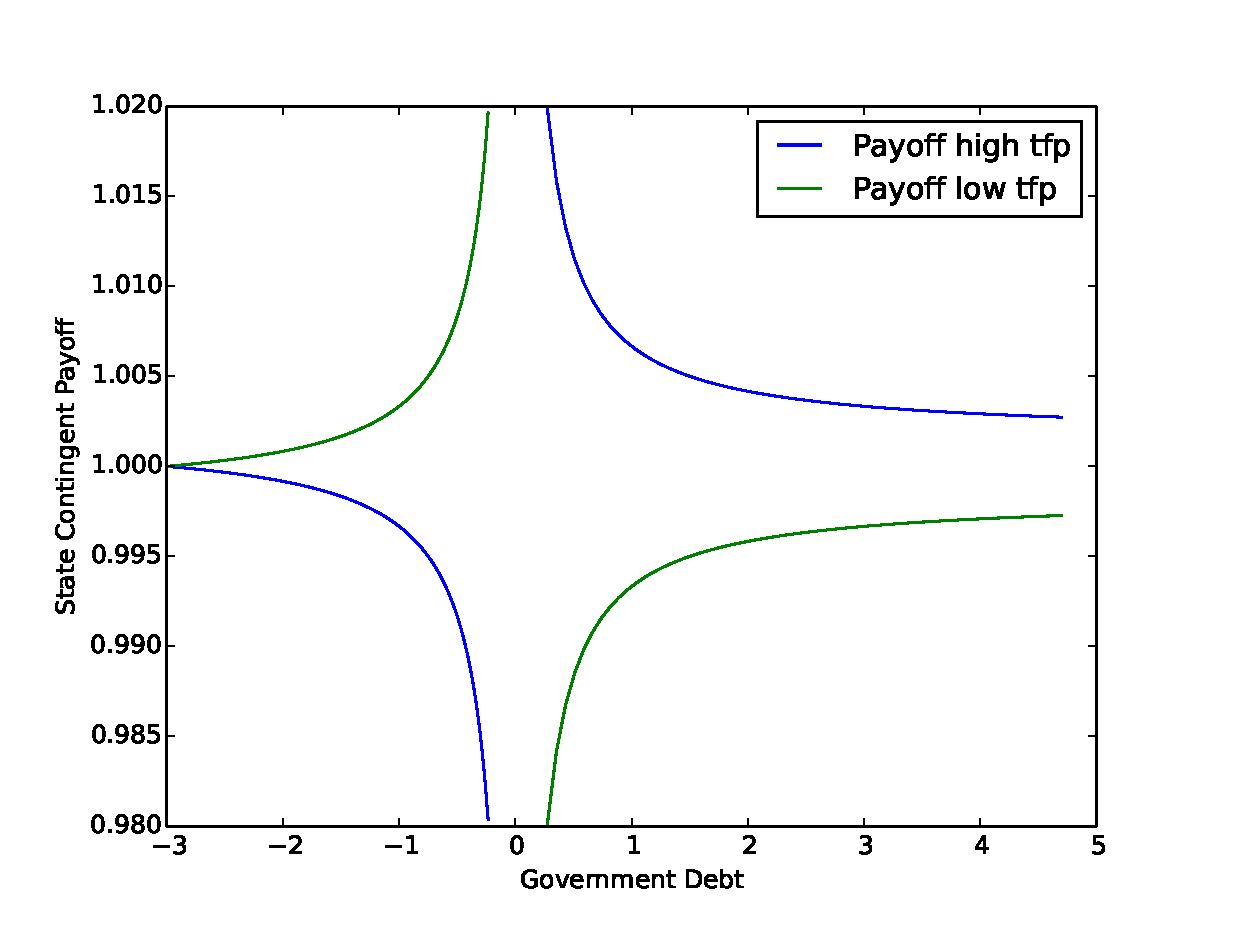
\includegraphics[scale=.4]{Images/p_graph_tfp.eps}
		\caption{Optimal asset payoff structure as a function of initial government debt when TFP follows a 2 shock i.i.d process}
	\end{center}	
	\end{figure}


\begin{figure}
		\begin{center}
		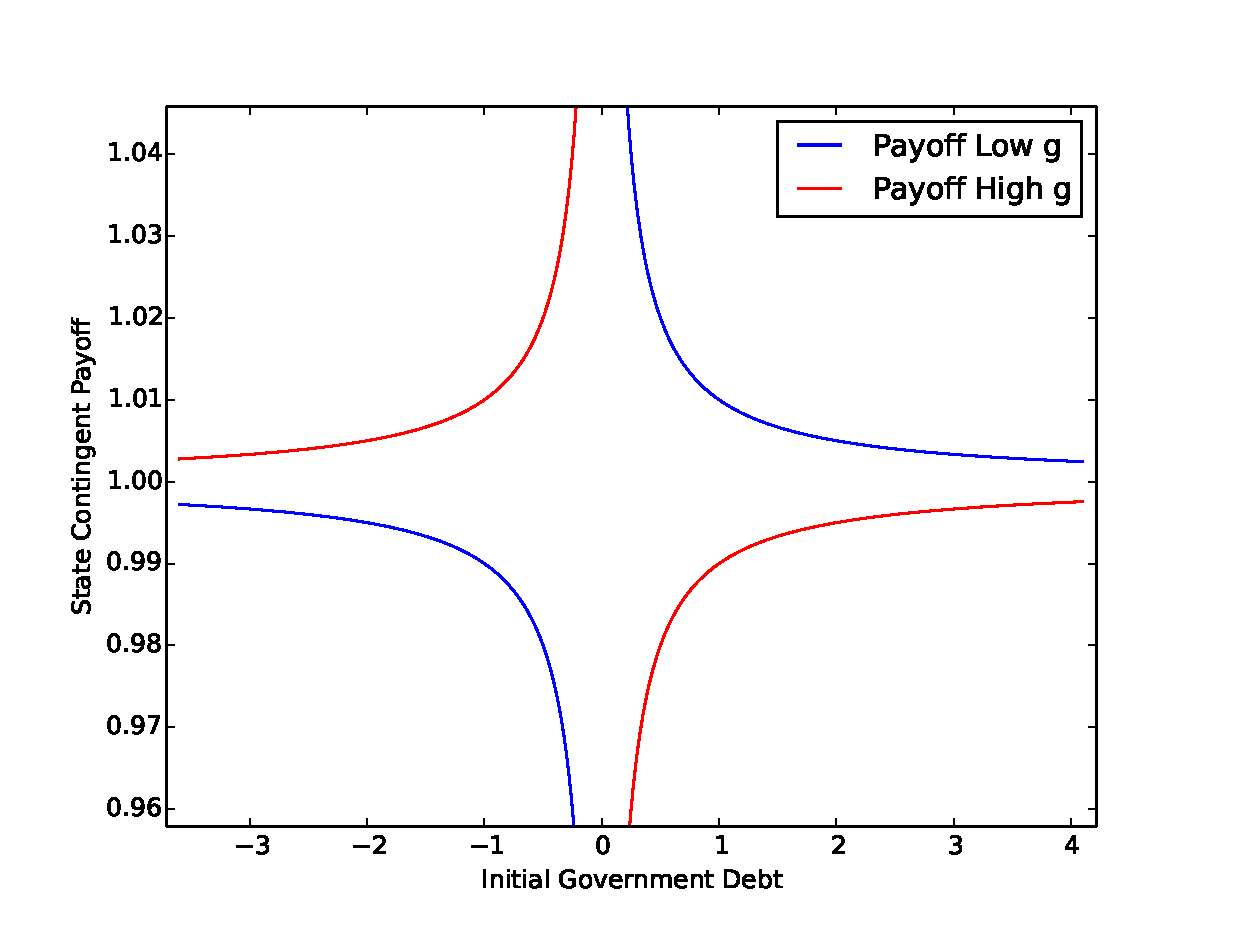
\includegraphics[scale=.4]{Images/p_graph.eps}
		\caption{Optimal asset payoff structure as a function of initial government debt when government expenditures follow 2 shock i.i.d process}
	\end{center}	
	\end{figure}


\begin{figure}
		\begin{center}
		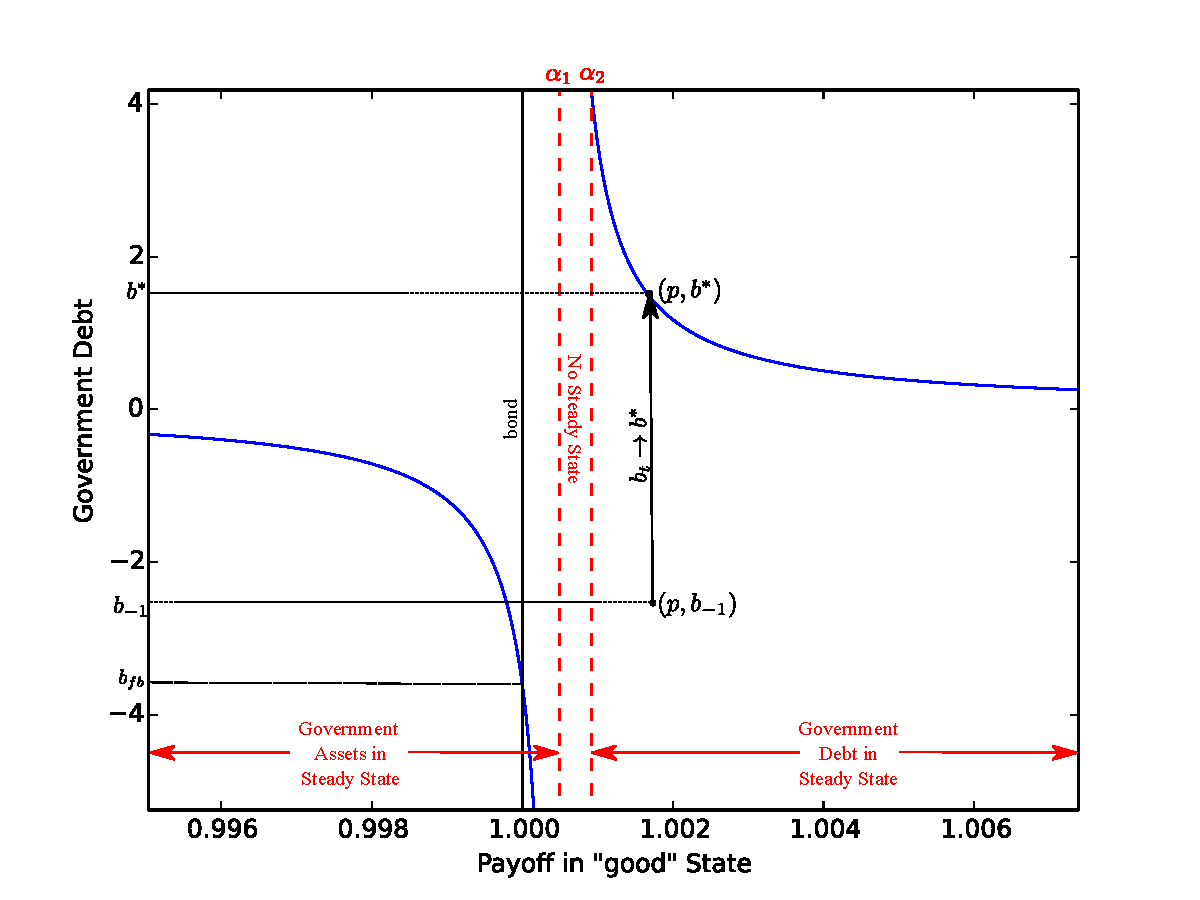
\includegraphics[width=4.2in]{Images/graph_nostable.pdf}
\caption{Existence regions in $\bm{p}$ space}
	\end{center}	
	\end{figure}



	\begin{figure}
		\begin{center}
		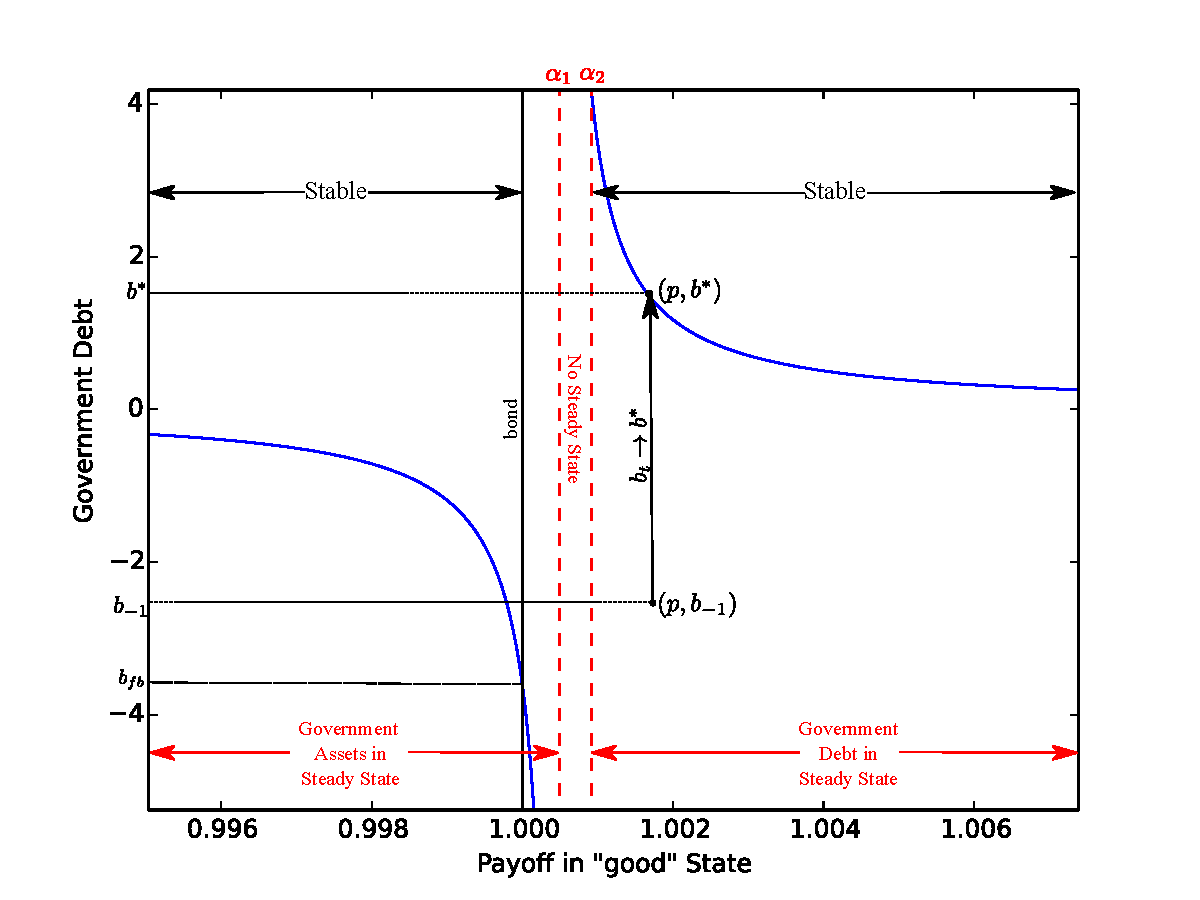
\includegraphics[width = 4.2in]{Images/graph_stable.pdf}
\caption{Stability regions}
	\end{center}	
	\end{figure}	

\begin{figure}
	\begin{center}
	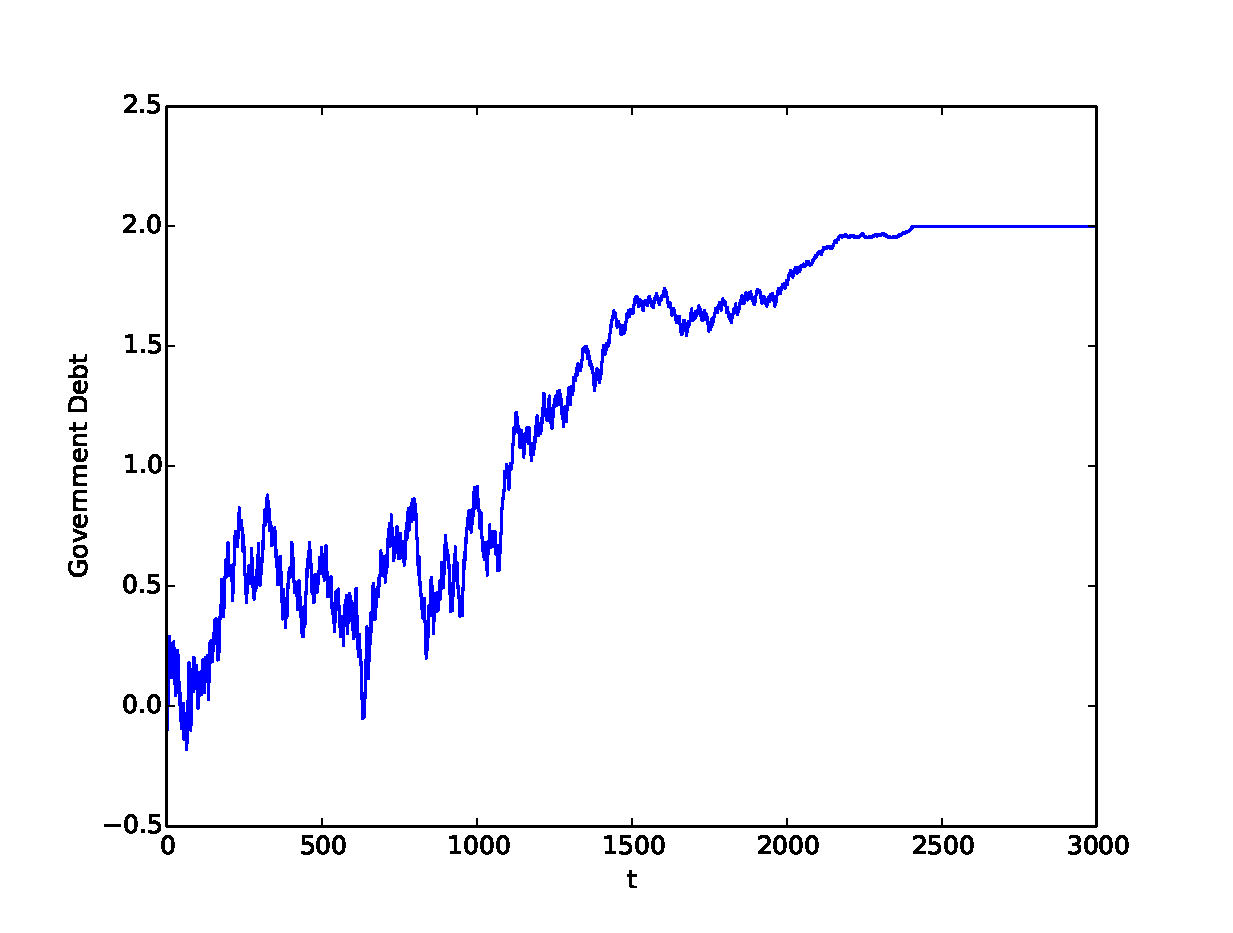
\includegraphics[width=4in]{Images/port1.eps}
    \caption{A sample path with  $\bm{p} > 1$}
	\end{center}
\end{figure}

\begin{figure}
	\begin{center}
	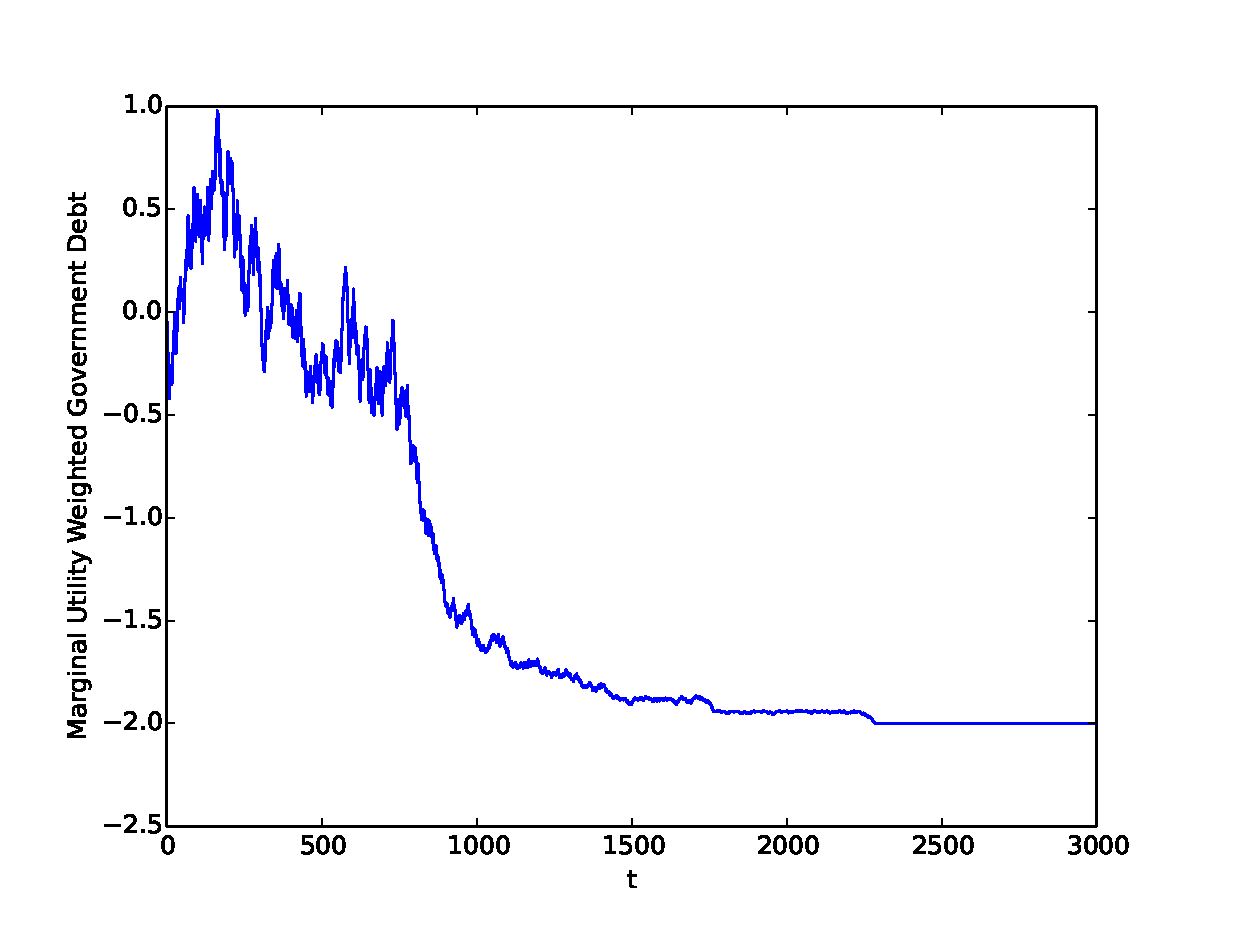
\includegraphics[width=4in]{Images/port2.eps}
\caption{A sample path with   $\bm{p} <1$}
	\end{center}	
\end{figure}



\begin{figure}
	\begin{center}
	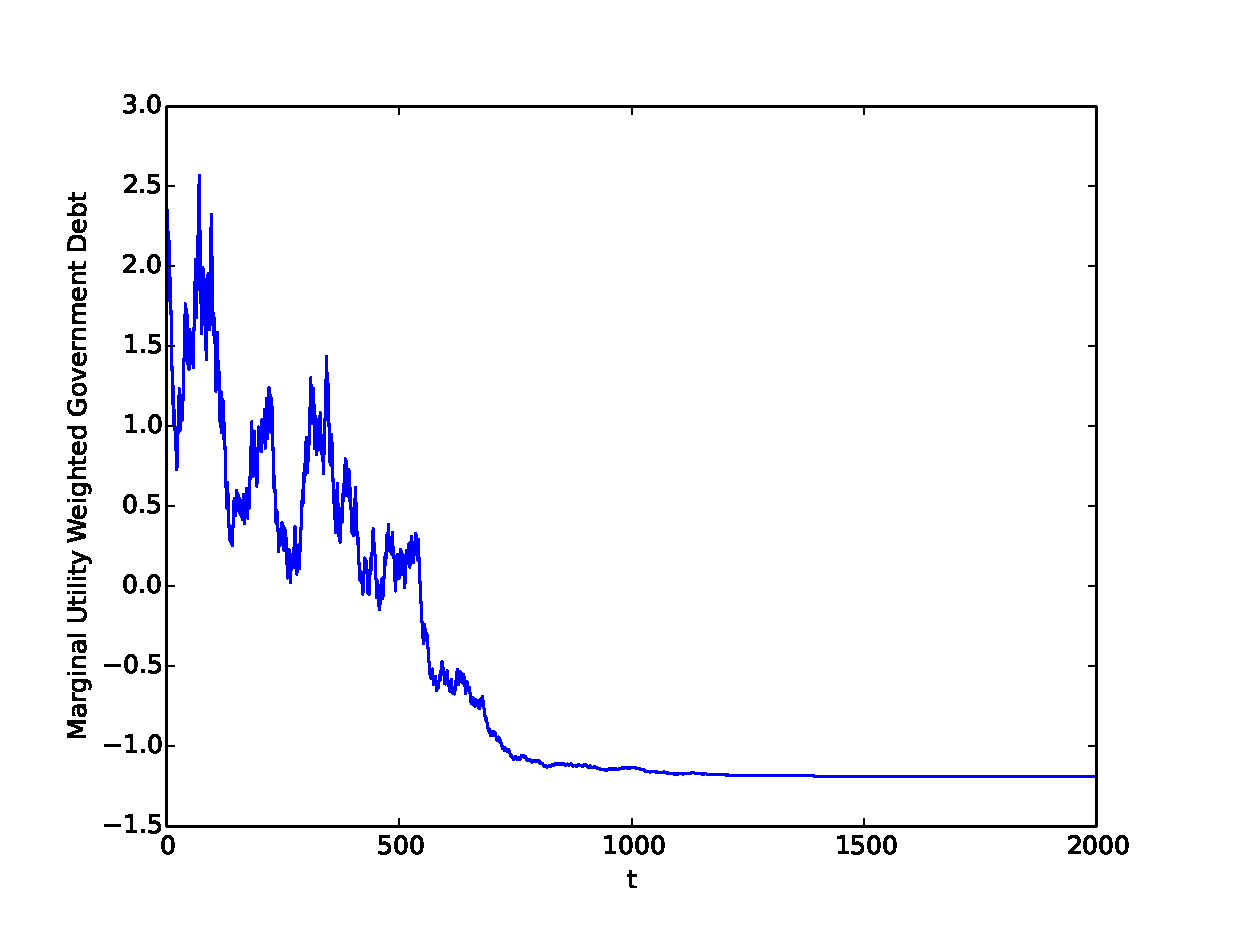
\includegraphics[width=4in]{Images/2stateiid.eps}
\caption{A sample path for 2 state i.i.d. process with risk aversion}
	\end{center}
\end{figure}


	\begin{figure}
	\begin{center}
	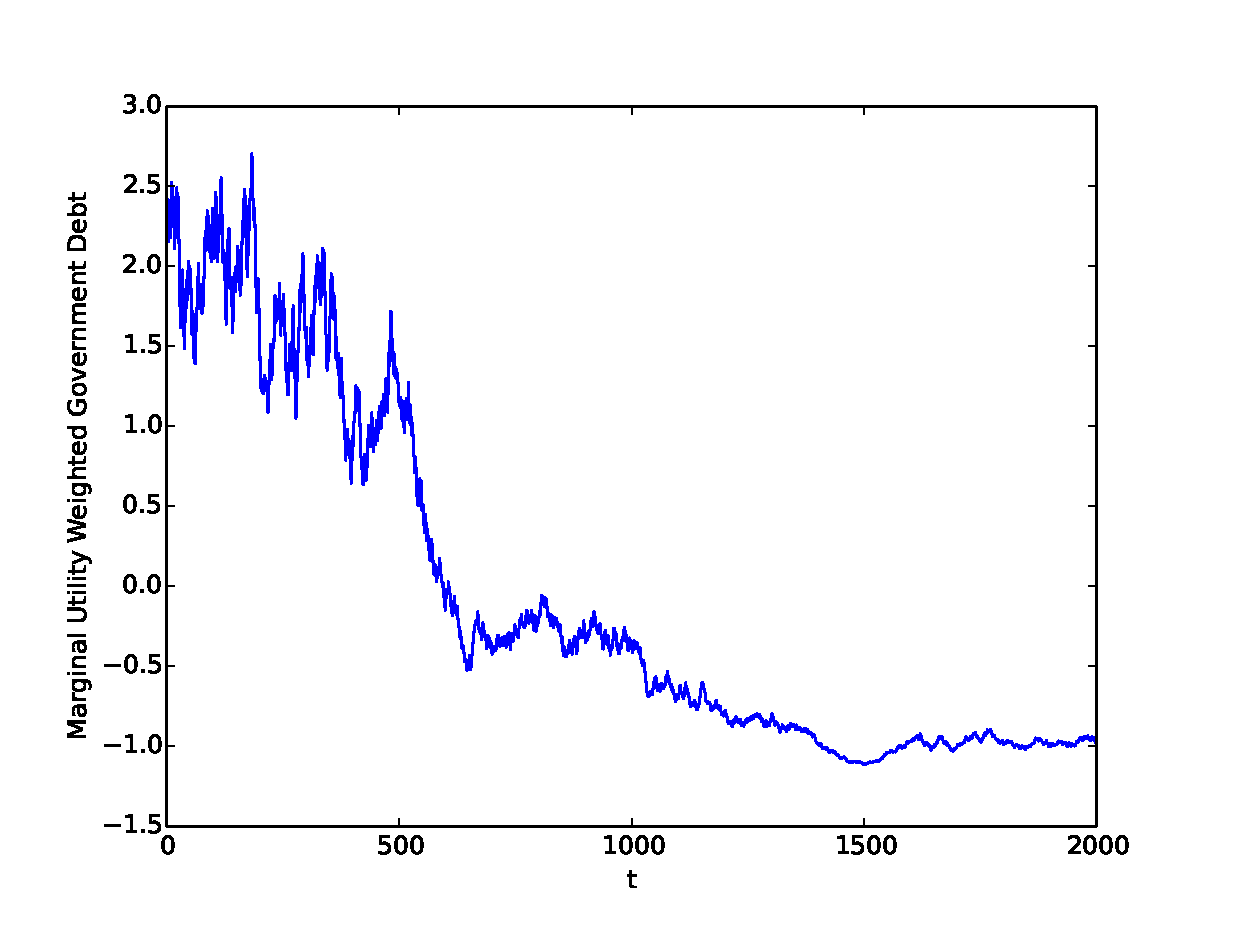
\includegraphics[width=4in]{Images/5stateiid.eps}
\caption{A sample path  for economy with $S>2$ states}
	\end{center}
\end{figure}



\begin{figure}
	\begin{center}
	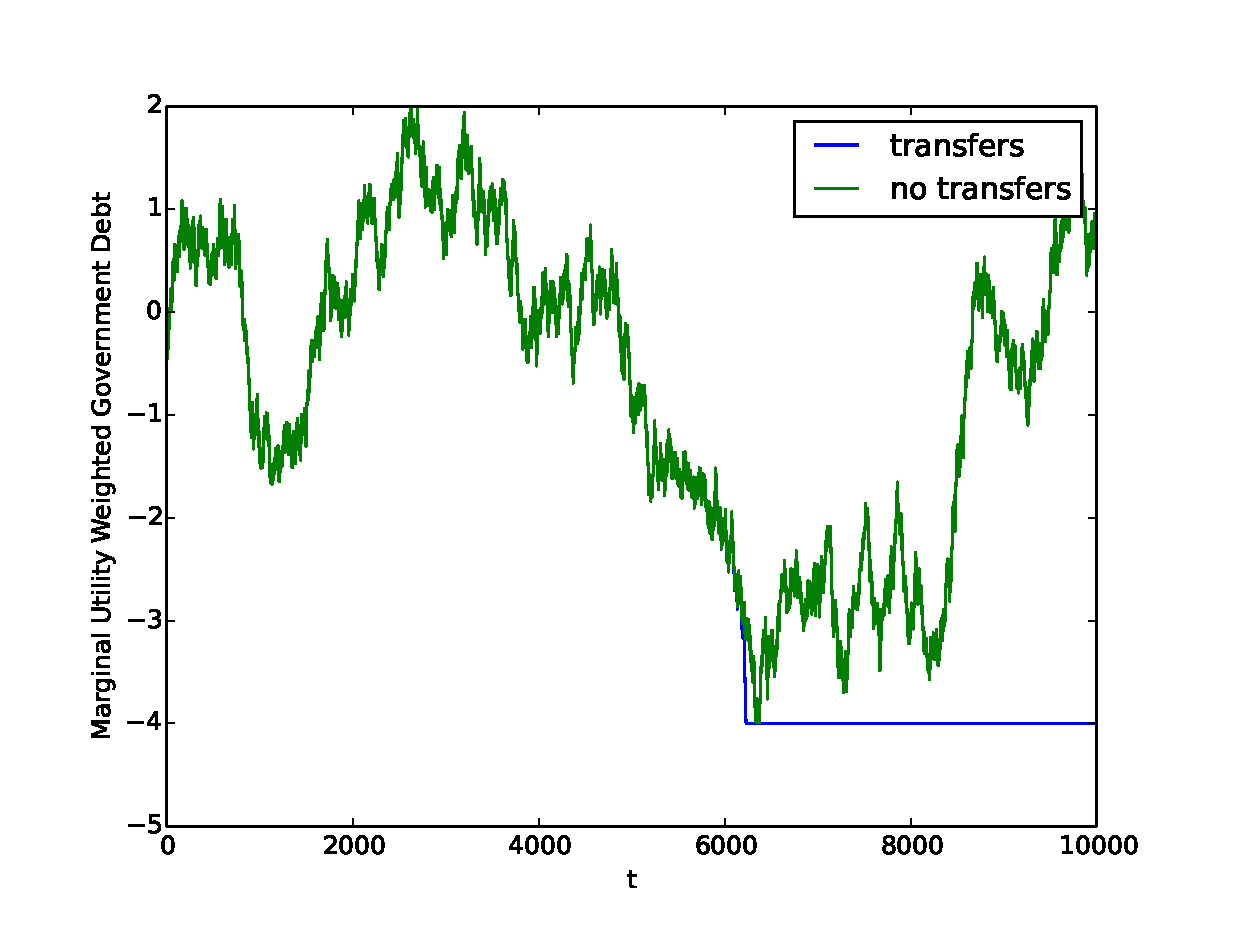
\includegraphics[width=4in]{Images/transfer_example2.eps}
\caption{Quasilinear preferences and risk-free bond  with and without nonnegative transfers}
	\end{center}
\end{figure}



 \end{enumerate}

\bibliography{BEGS}

\end{document}
